\documentclass{article}\usepackage[]{graphicx}\usepackage[]{color}
%% maxwidth is the original width if it is less than linewidth
%% otherwise use linewidth (to make sure the graphics do not exceed the margin)
\makeatletter
\def\maxwidth{ %
  \ifdim\Gin@nat@width>\linewidth
    \linewidth
  \else
    \Gin@nat@width
  \fi
}
\makeatother

\definecolor{fgcolor}{rgb}{0.514, 0.58, 0.588}
\newcommand{\hlnum}[1]{\textcolor[rgb]{0.863,0.196,0.184}{#1}}%
\newcommand{\hlstr}[1]{\textcolor[rgb]{0.863,0.196,0.184}{#1}}%
\newcommand{\hlcom}[1]{\textcolor[rgb]{0.345,0.431,0.459}{#1}}%
\newcommand{\hlopt}[1]{\textcolor[rgb]{0.576,0.631,0.631}{#1}}%
\newcommand{\hlstd}[1]{\textcolor[rgb]{0.514,0.58,0.588}{#1}}%
\newcommand{\hlkwa}[1]{\textcolor[rgb]{0.796,0.294,0.086}{#1}}%
\newcommand{\hlkwb}[1]{\textcolor[rgb]{0.522,0.6,0}{#1}}%
\newcommand{\hlkwc}[1]{\textcolor[rgb]{0.796,0.294,0.086}{#1}}%
\newcommand{\hlkwd}[1]{\textcolor[rgb]{0.576,0.631,0.631}{#1}}%

\usepackage{framed}
\makeatletter
\newenvironment{kframe}{%
 \def\at@end@of@kframe{}%
 \ifinner\ifhmode%
  \def\at@end@of@kframe{\end{minipage}}%
  \begin{minipage}{\columnwidth}%
 \fi\fi%
 \def\FrameCommand##1{\hskip\@totalleftmargin \hskip-\fboxsep
 \colorbox{shadecolor}{##1}\hskip-\fboxsep
     % There is no \\@totalrightmargin, so:
     \hskip-\linewidth \hskip-\@totalleftmargin \hskip\columnwidth}%
 \MakeFramed {\advance\hsize-\width
   \@totalleftmargin\z@ \linewidth\hsize
   \@setminipage}}%
 {\par\unskip\endMakeFramed%
 \at@end@of@kframe}
\makeatother

\definecolor{shadecolor}{rgb}{.97, .97, .97}
\definecolor{messagecolor}{rgb}{0, 0, 0}
\definecolor{warningcolor}{rgb}{1, 0, 1}
\definecolor{errorcolor}{rgb}{1, 0, 0}
\newenvironment{knitrout}{}{} % an empty environment to be redefined in TeX

\usepackage{alltt}
\usepackage{geometry}
\geometry{verbose, tmargin=2.5cm, bmargin=2.5cm, lmargin=2.5cm, rmargin=2.5cm}
\IfFileExists{upquote.sty}{\usepackage{upquote}}{}
\begin{document}

\title{Minimal Empirical Density Estimation}
\author{Matthew Leonawicz}
\maketitle





\section{Simulation results}



The first plot shows a histogram of the original simulated data, overlain with boostrap resamples drawn from the crudely estimated density, and finally, a new density estimation performed post-bootstrap.
The second plot shows the same, but incorporates an intermediary step involving linear approximation.
This allows the subsequent draws to be more continuous.

\begin{knitrout}
\definecolor{shadecolor}{rgb}{0, 0.169, 0.212}\color{fgcolor}
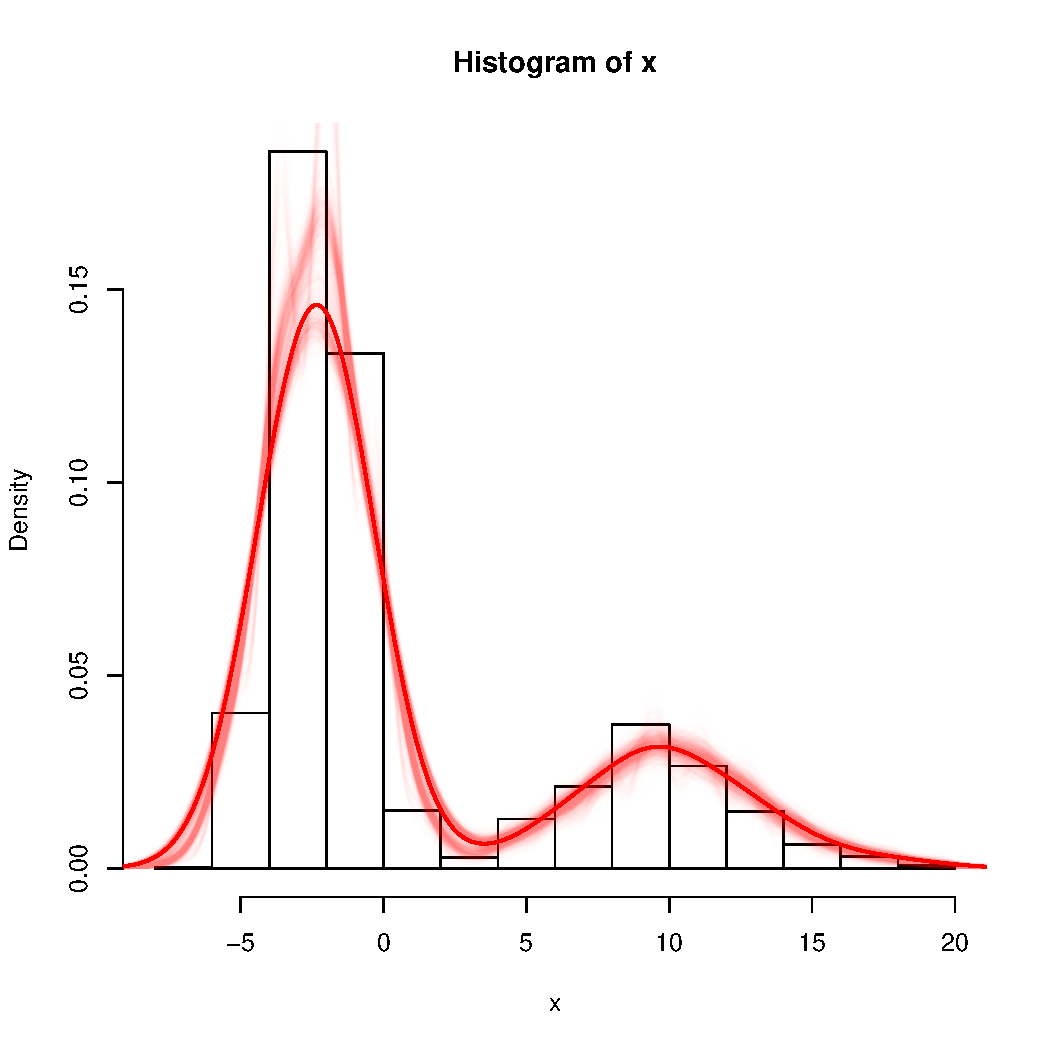
\includegraphics[width=\maxwidth]{figure/plot1-1} 

\end{knitrout}

\begin{knitrout}
\definecolor{shadecolor}{rgb}{0, 0.169, 0.212}\color{fgcolor}
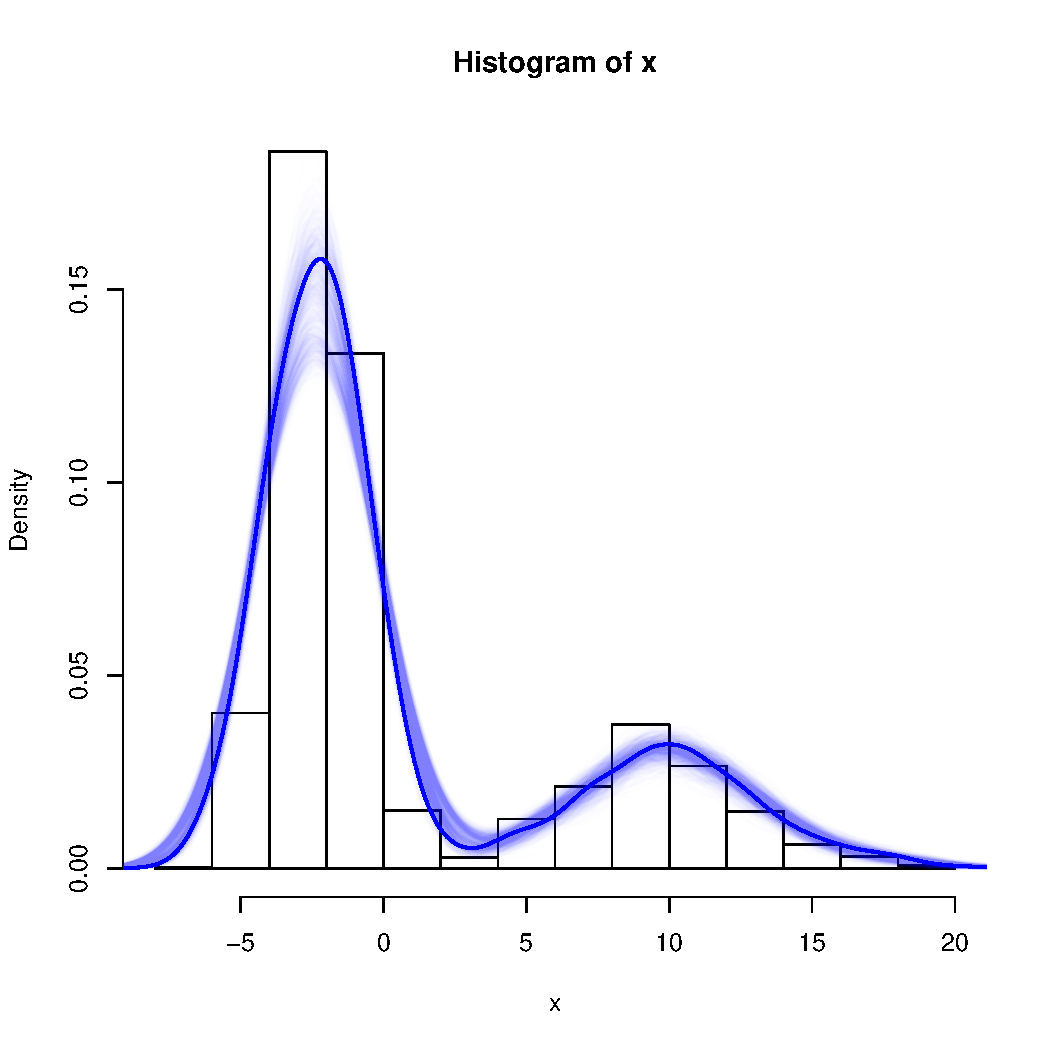
\includegraphics[width=\maxwidth]{figure/plot2-1} 

\end{knitrout}

\end{document}
